% \secrel{Маркировка моделей станков производства СССР}
% 
% \begin{tabular}{p{0.3\textwidth} p{0.6\textwidth}}
% 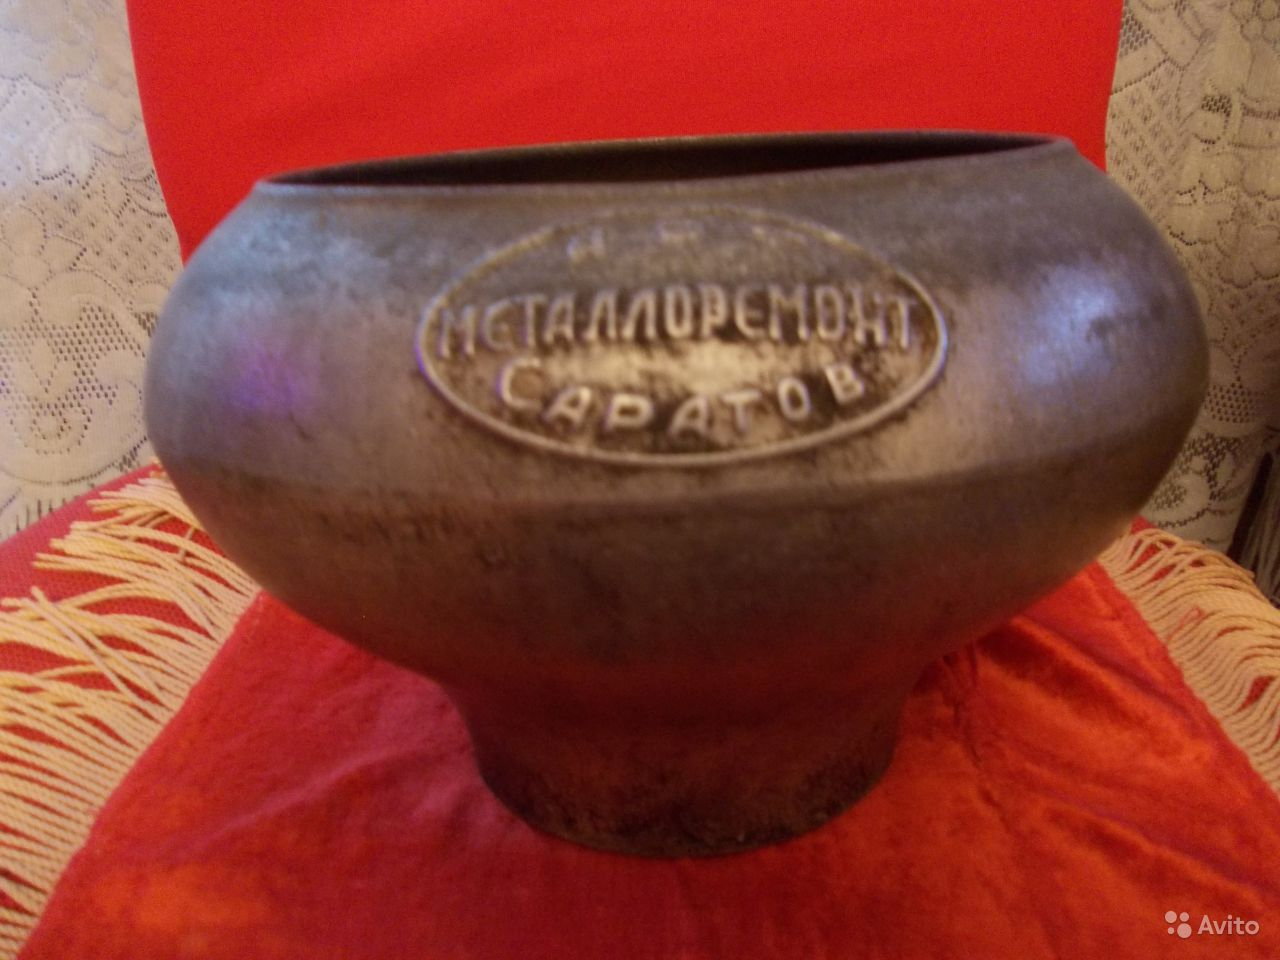
\includegraphics[height=0.3\textheight]{stanki/chugunok.jpg}
% &
% станок-''чугунок'', простой, дубовый, надежный (потому что ненадежные давно
% сломались), дешевый, но требует помещение с силовым полом, 3х-фазное питание, и
% кучу времени на поиск запчастей для восстановления по металлобазам и развалам. В
% диком виде пока что встречается в школах и других типа учебных заведениях, т.к.
% висит на балансе, но не эксплуатируется, и не обслуживается, потому что некем.
% Отличается дешевизной (ржавого) инструмента и (еще более ржавой) оснастки, и
% некоторым гемором с поиском запчастей.
% \\
% \end{tabular}
% \clearpage
% 
% Для станков, выпускавшихся в СССР, принята единая система классификации и
% условных обозначений, основанная на присвоении каждому станку особого шифра
% (номера). Cтанки каждой группы подразделяются на девять \emph{типов}.
% Внутри каждого типа металлорежущие станки могут отличаться друг от друга
% конструктивными особенностями. Эти особенности, а также некоторые другие
% характеристики и отражаются в шифре (номере) станка.
% 
% \begin{verbatim}
% <группа>[<буква1>]<тип><характеризующий размер>[<буква2>][M][Фn]
% \end{verbatim}
% 
% Кроме цифр, в условные обозначения модели станка часто входят буквы. Если
% \emph{буква1} стоит между первой и второй цифрами, то это означает, что
% конструкция станка подверглась усовершенствованию по сравнению с прежней
% моделью.
% 
% Если \emph{буква2} стоит в конце номера станка, то это говорит об
% изменении основной, «базовой» модели станка. Часто \emph{буква2} задает класс
% точности:
% 
% \begin{description}
% \item[Н] нормальная (часто не указывается)
% \item[П] повышенная
% \item[В] высокая
% \item[А] особо высокая
% \item[С] особо-точный станок
% \end{description}
% 
% Для станков с ЧПУ:
% \begin{description}
% \item[М] наличие магазина инструментов,
% \item[Ф1] станки с цифровой индикацией и преднабором координат,
% \item[Ф2] с позиционными и прямоугольными системами,
% \item[Ф3] с контурными системами,
% \item[Ф4] с универсальной системой для позиционной и контурной обработки. Эти
% шифры пишутся в конце номера модели.
% \end{description}
% 
% \bigskip
% \noindent\emph{группа}/\emph{тип}:
% \begin{enumerate}[label={\arabic*}]
%   \item токарные;
%   \begin{enumerate}[label={\arabic*}]
%     \item
%     \item
%     \item револьверные;
%     \item
%     \item
%     \item токарно-винторезные;
%   \end{enumerate}
%   \item сверлильные и расточные;
%   \begin{enumerate}[label={\arabic*}]
%     \item вертикально-сверлильные,
%     \item одношпиндельные полуавтоматы,
%     \item многошпиндельные полуавтоматы,
%     \item координатно-расточные,
%     \item радиально-сверлильные,
%     \item горизонтально-расточные,
%     \item алмазно-расточные,
%     \item горизонтально-сверлильные,
%     \item разные сверлильные.
%   \end{enumerate}
%   \item шлифовальные, полировальные, доводочные и заточные;
%   \item специальные;
%   \item зубо- и резьбообрабатывающие;
%   \item фрезерные;
%   \item разрезные;
%   \item строгальные, долбежные, протяжные;
%   \item прочие
% \end{enumerate}
% 
% \bigskip
% \term{Характеризующий размер}:
% \begin{description}
% \item[токарные] \hfill \\
% высота оси шпинделя над станиной, \\
% задает \emph{максимально возможный радиус} обрабатываемой \emph{заготовки}
% \end{description}
% 
% \bigskip
% Пример: 1А616: станок токарно(1)-винторезный(6), модификация(А), высота
% центров над станиной (16)0 мм.
